\section{Compatible seeds, geometric doubling, and sparse families}
\label{fam:section}

The second extension mechanism inserts a whole collection of lines near
a distinguished support.  It belongs to Bartholdi, Blanc, and Loisel
(BBL)~\cite{bbl2008}; it is fundamentally different from the one-line
exterior operation of Section~\ref{ext:section}.  The present work supplies
explicit compatible seeds, a recursively closed geometric Lean proof, and
finite certificates at considerably larger orders. The October release
completes both the odd iteration and the stronger adjacent-even family.
The numerical doubling gain retains its published attribution.

\subsection{The exact one-step theorem}

Let $q=4r$ with $r\geq5$, put $\alpha=\pi/q$, and take
\begin{equation}
  0<\varepsilon<\tan(\alpha/2).
  \label{fam:epsilon}
\end{equation}
Define $q$ ordered intercepts, indexed from zero, by
\begin{equation}
 a_j=
 \begin{cases}
 \tan((j-q/2+1)\alpha),&0\leq j<q/2-1,\\
 -\varepsilon,&j=q/2-1,\\
 \varepsilon,&j=q/2,\\
 \tan((j-q/2)\alpha),&q/2<j<q.
 \end{cases}
 \label{fam:old-grid}
\end{equation}
In particular, the extreme intercepts are $-\cot\alpha$ and
$\cot\alpha$.  The two central intercepts replace the repeated zero that
would otherwise occur in this grid.

\begin{definition}[Compatible tangent-grid seed]
\label{fam:compatible}
A seed at $(q,\varepsilon)$ consists of $Y_0:y=0$ and the $q$ lines
$L_j:y=m_j(x-a_j)$, with the following properties: the arrangement is
simple; every interval $[a_j,a_{j+1}]$ on $Y_0$ supports the triangular
cell with supports $Y_0,L_j,L_{j+1}$; and the central apex
$L_{q/2-1}\cap L_{q/2}$ lies above $Y_0$.  A counted seed additionally
carries a list of distinct actual triangular cells whose length is at
least $T$.
\end{definition}

Simplicity already requires all $m_j$ to be nonzero and pairwise distinct.
The distinguished-line condition is a substantial geometric restriction,
not a consequence of having a large total count.  It is precisely why
an arbitrary optimal arrangement cannot simply be used as a repeatable
BBL seed.

\begin{theorem}[Fully verified geometric doubling]
\label{fam:doubling}
Suppose $q=4r\geq20$ and \eqref{fam:epsilon} holds.  A compatible
tangent-grid seed with at least $T$ certified triangles gives a simple
real straight-line arrangement of $2q+1$ lines with at least
\begin{equation}
  T+q^2
  \label{fam:gain}
\end{equation}
triangles.
\end{theorem}

The precise formal theorem is \texttt{BBLDoubling.doubling}.  It assumes
the actual old line equations, simplicity, each distinguished triangle,
the positive central height, and a duplicate-free triangle list.  It
does not assume a future crossing order, a list of future empty
triangles, or a triangle-count recurrence.  Its conclusion is an actual
\texttt{SimpleLowerBound}; the generic proof uses only the standard Lean
logical axioms.  The numerical doubling principle is BBL's.  The
contribution here is its completed geometric proof for these explicit
hypotheses, using the following two-parameter realization.

\begin{proof}[Geometric proof and its formal decomposition]
For $0\leq i<q$ set
\[
 \beta_i=-\frac\pi2+(i+\tfrac12)\alpha,
 \qquad b_i=\tan\beta_i.
\]
Adjoin the lines
\begin{equation}
 M_i:\quad y=\kappa g_i(\delta)(x-b_i),\qquad
 g_i(\delta)=\frac{2b_i}{1+b_i^2}+\frac\delta{b_i}
            =\sin(2\beta_i)+\delta\cot\beta_i.
 \label{fam:pencil}
\end{equation}
Choose $\delta>0$ sufficiently small and then $\kappa>0$ sufficiently
small relative to the fixed $\delta$ and the seed.  This order of choices
is part of the proof.  BBL's published construction uses explicit scales;
the qualitative two-scale statement here is established independently
by the formal crossing analysis, rather than inferred from those fixed
scales.

For two new lines put $t=b_i$ and $u=b_k$.  Their intersection has
$x$-coordinate independent of $\kappa$:
\begin{equation}
 X_{ik}(\delta)=
 \frac{2tu(t+u)}{2tu(1-tu)-\delta(1+t^2)(1+u^2)}.
 \label{fam:crossing}
\end{equation}
When $tu\ne1$, its limit is the reduced tangent
$(t+u)/(1-tu)=\tan(\beta_i+\beta_k)$, and the exact displacement is
\begin{equation}
 X_{ik}(\delta)-\frac{t+u}{1-tu}
 =\frac{\delta(t+u)(1+t^2)(1+u^2)}
 {[2tu(1-tu)-\delta(1+t^2)(1+u^2)](1-tu)}.
 \label{fam:displacement}
\end{equation}
For sufficiently small positive $\delta$ its nonzero sign is that of
$(t+u)tu$.  If $tu=1$, the crossing diverges along the specified exterior
ray as $\delta\downarrow0$; if $t+u=0$, its coordinate is exactly zero.
Thus neither exceptional case is hidden inside a continuity argument
with a vanishing denominator.

The reduced tangents, the old intercepts, the new half-grid intercepts,
and $-\varepsilon,0,\varepsilon$ determine a strictly ordered finite
system of cuts.  Equations~\eqref{fam:crossing}--\eqref{fam:displacement}
place every new--new crossing in its prescribed cut interval.  Taking
$\delta$ in the intersection of the finitely many resulting positive
neighborhoods also makes the new slope factors nonzero and distinct.
For fixed such $\delta$, each old--new intersection tends to the
corresponding old intercept as $\kappa\to0$.  Finite continuity then
realizes all the prescribed strict crossing comparisons simultaneously.
Small $\kappa$ separates old and new slopes.  Injectivity along each new
crossing row excludes new triple intersections; old simplicity excludes
the remaining ones.  This proves actual simplicity and crossing order.

The count can now be separated from trigonometry.  Treat the $q$ new lines
and $Y_0$ as $q+1$ auxiliary supports.  The integer row model places old
support $j$ at key $4j+2$.  A pair of auxiliary supports with crossing key
$z$ yields a mixed triangle with old support $j$ when
\begin{equation}
  |z-(4j+2)|<4.
  \label{fam:neighbors}
\end{equation}
Every auxiliary pair has two such old neighbors, except for at most $q$
exterior pairs, each of which has one.  Hence the number is at least
\begin{equation}
 2\binom{q+1}{2}-q=q^2.
 \label{fam:mixed-count}
\end{equation}
The row inequalities make two sides consecutive on their supports.
The two-side emptiness lemma proves that the corresponding triangle is
an actual empty cell.  The supporting triples are distinct.  Thus
\eqref{fam:mixed-count} counts genuine triangles, not merely local
crossing patterns.

It remains to preserve the seed's contribution.  An old triangle not
using $Y_0$ has a strict half-plane sign against $Y_0$; all new lines
converge to $Y_0$, so its three vertex signs persist for sufficiently
small $\kappa$.  The old triangles with a side on $Y_0$ require a different
argument.  Saturation forces consecutive old apices to have opposite
heights.  The positive central apex fixes the alternating parity.
The crossing order identifies a new cap support for each noncentral
distinguished triangle.  On both cap endpoints, every new line has the
parity-correct weak sign; strict signs against other old supports
persist by continuity.  This replaces each such old triangle by one
empty triangle with the same two old supports.  The central triangle
itself is retained.  The finite cap and noncap requirements can again
be satisfied by one common positive $\kappa$.

Finally, these $T$ retained or replaced triangles have at least two old
nonhorizontal supports, while the $q^2$ mixed triangles have two
auxiliary supports.  The supporting triples cannot coincide.  Their
union is a duplicate-free witness of length at least $T+q^2$.
\end{proof}

The recurrence preserves the certified segment deficit:
\begin{equation}
 \Delta(q,T)=q^2-1-3T,\qquad
 \Delta(2q,T+q^2)=\Delta(q,T).
 \label{fam:deficit-preserved}
\end{equation}
Here the equality concerns the transported lower count; if the output
has additional uncounted triangles, its actual defect can be smaller.
Thus doubling amplifies a compatible seed to larger orders while
preserving its certified constant deficit.  A smaller-defect seed or a
new source of additional triangles is needed to improve that deficit.

\subsection{The compatible eleven-line realization}

The useful eleven-line count is $32$, an existing result; the search
started from the Honma-based construction displayed by
Savchuk~\cite{savchuk2025}.  The additional work here is an explicit
realization compatible with the BBL grid for arbitrarily small positive
central separation.  Take $Y_0:y=0$ and
\begin{equation}
 x-v_jy=a_j,\qquad
 (v_0,\ldots,v_9)=\tfrac1{10}(15,-2,14,1,4,-4,5,-3,12,-5),
 \label{fam:seed11-slopes}
\end{equation}
where
\begin{equation}
 (a_0,\ldots,a_9)=
 (-\tan\tfrac{4\pi}{10},-\tan\tfrac{3\pi}{10},
 -\tan\tfrac{2\pi}{10},-\tan\tfrac{\pi}{10},
 -\varepsilon,\varepsilon,
 \tan\tfrac{\pi}{10},\tan\tfrac{2\pi}{10},
 \tan\tfrac{3\pi}{10},\tan\tfrac{4\pi}{10}).
 \label{fam:seed11-grid}
\end{equation}
For every $0<\varepsilon\leq10^{-5}$ the seed is simple, has at least
32 certified triangles, and has all nine distinguished triangles.
Its central slopes are $5/2$ and $-5/2$ and its central height is
$5\varepsilon/2>0$.

The stability check is finite but uniform in $\varepsilon$.  The
determinant for a triple of nonhorizontal lines is affine in the
intercepts and therefore affine in $\varepsilon$:
\[
 D_{ijk}=(a_j-a_k)v_i+(a_k-a_i)v_j+(a_i-a_j)v_k.
\]
Exact rational enclosures for the four tangent values and endpoint
sign checks certify the whole interval.  The first certificate used
outward rational interval arithmetic; the subsequent Lean theorem uses
proved trigonometric enclosures and the parametric certificate soundness
theorem.  The limit $\varepsilon=0$ is used only to bound expressions;
it is not presented as a simple arrangement.  Five visible pairs for
$w=(10,-13)$ are also proved uniformly, giving the actual exterior bound
$12:37$ by Theorem~\ref{ext:realization}.

\begin{figure}[tb]
\centering
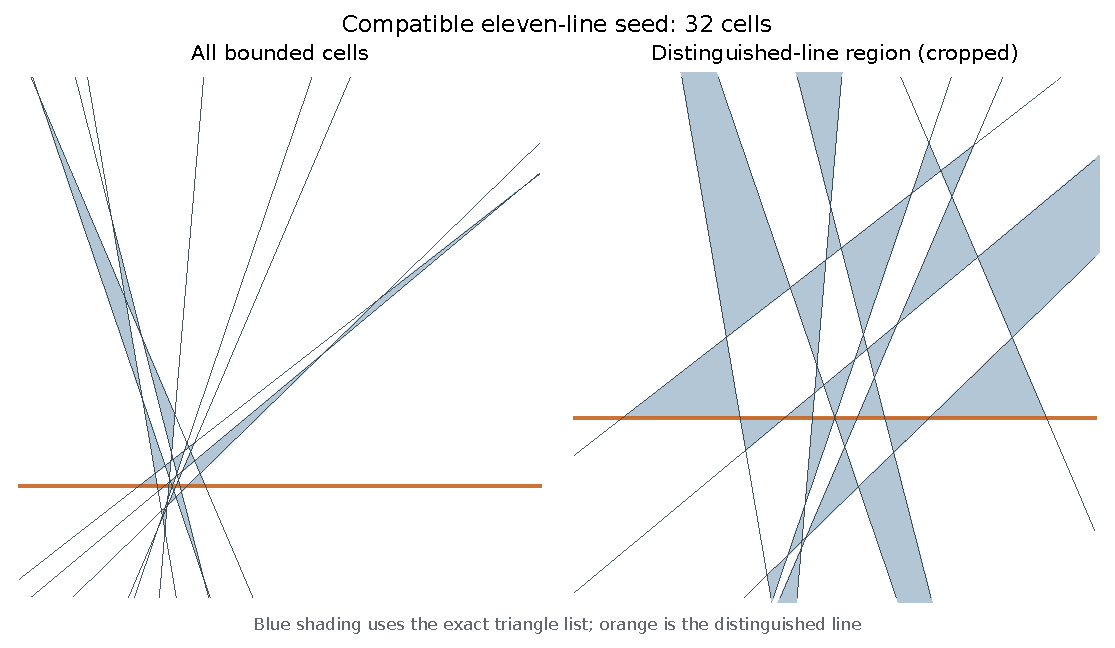
\includegraphics[width=0.88\linewidth]{figures/seed-11.pdf}
\caption{A finite rational realization of the compatible eleven-line
seed, with global and distinguished-line views.  The figure illustrates
the arrangement; the all-small-parameter
claim is certified by exact determinant and half-plane inequalities,
not by the rendering.  The count $32$ is inherited from earlier work;
the compatible realization and parameter certificate are the contribution
recorded here.}
\label{fig:seed11}
\end{figure}

\subsection{Closing the geometric invariant}

A numerical inequality after one step is insufficient for induction. The
output must again satisfy every geometric hypothesis in
Definition~\ref{fam:compatible}. The October construction returns precisely
that information. The \proofref{Kobon/BBLRecursiveSeed.lean}{11}{seed record}
contains actual slopes, a duplicate-free valid triangle list, simplicity,
every consecutive distinguished triangle, and the positive central apex.
The line labels are normalized by explicit inverse permutations; the
transport theorem preserves actual support triples and their triangle
predicates, rather than merely transporting a count.

\begin{theorem}[Closed geometric iteration]\label{fam:closed-iteration}
Fix $r\ge5$ and a counted seed size $T$. Suppose that for every sufficiently
small positive $\varepsilon$ a compatible tangent-grid seed with $4r+1$
lines and at least $T$ triangles exists. Then for every integer $t\ge0$
there is a simple arrangement of $4r\,2^t+1$ lines with at least $T_t$
triangles, where
\begin{equation}
 T_0=T,\qquad T_{t+1}=T_t+(4r\,2^t)^2,
 \qquad 3T_t+(4r)^2=3T+(4r\,2^t)^2.
 \label{fam:closed-count}
\end{equation}
At every finite depth the full seed invariant is available on some
nonempty positive parameter interval.
\end{theorem}

\begin{proof}
The geometric construction in Theorem~\ref{fam:doubling} is performed
while retaining the next distinguished triangles and the positive central
triangle. Its output intercepts, after the proved reindexing, are exactly
the tangent grid for $2r$. Simplicity and the counted list are carried in
the same witness. This is
\proofref{Kobon/BBLRecursiveSeed.lean}{61}{\lean{seed_step}}; its
coefficient identities are proved in \lean{BBLRecursiveGrid} and its
unreindexed geometric witness in \lean{BBLRecursiveWitness}.

More explicitly, let $\eta>0$ be a valid input threshold. The next seed
exists for every
\[
 0<\varepsilon<\min\{\eta,\tan(\pi/(8r))\}.
\]
The minimum is positive. For each such $\varepsilon$, the small pencil
parameters are chosen as in the one-step proof. No uniform lower bound
on these auxiliary parameters is needed. Thus the whole seed property,
including its nonempty interval, is preserved by $r\mapsto2r$.
Induction proves the first assertion and the recurrence. Multiplying
the recurrence by three and using $(2q)^2=q^2+3q^2$ proves the displayed
identity by induction. The formal results are
\proofref{Kobon/BBLInfinite.lean}{32}{\lean{uniform_iterate}},
\proofref{Kobon/BBLInfinite.lean}{46}{\lean{infinite_family}}, and
\proofref{Kobon/BBLInfinite.lean}{52}{\lean{triangleCount_identity}}.
\end{proof}

The quantifier is $\forall t\,\exists\eta_t>0\,\forall\varepsilon
\in(0,\eta_t)$, with a seed witness for each such parameter. It is not
$\exists\varepsilon>0\,\forall t$. In particular, the theorem does not
claim that a fixed drawn arrangement can be iterated with one fixed
positive gap forever. This distinction closes the earlier proof gap
without inserting an unproved compactness assertion.

The normalized 21-line seed supplies $r=5$, $T=132$ throughout
$0<\varepsilon\le10^{-5}$. Its nineteen distinguished triangles, actual
coefficient identity, and central height $5\varepsilon/2$ are proved in
\lean{BBLSeed21Normalized}. The generic theorem starts at $r\ge5$;
the separately verified eleven-line seed supplies the initial term in
the following family.

\begin{theorem}[Verified odd family]\label{fam:odd-verified}
For every integer $t\ge0$, set $q_t=10\cdot2^t$. Then
\begin{equation}
 \Ks(q_t+1)\ge T_t=\frac{100\cdot4^t-4}{3}
                    =\frac{q_t^2-4}{3}.
 \label{fam:eleven-family}
\end{equation}
\end{theorem}
\begin{proof}
For $t=0$ use the eleven-line certificate. For $t\ge1$ apply
Theorem~\ref{fam:closed-iteration} to the normalized 21-line seed at depth
$t-1$. Equation~\eqref{fam:closed-count} gives $3T_t+4=q_t^2$.
The exact formal declaration is
\proofref{Kobon/BBLVerifiedFamilies.lean}{24}{\lean{eleven_odd_family}}.
\end{proof}

The generic iteration uses only standard logical axioms. The concrete
family additionally inherits four existing native certificate checks
from its 21-line base. This is an unconditional geometric existence
theorem with an explicitly reported computation trust boundary, not a
conditional recurrence on unknown arrangements.

\subsection{Even companions and the retained boundary invariant}

The defect argument of Theorem~\ref{ext:defect-theorem} gives the weaker
ordinary mathematical consequence
\begin{equation}
 \Ks(q+2)\ge\frac{q^2-4}{3}+\frac q2-1,
 \qquad q=10\cdot2^t.
 \label{fam:even-defect}
\end{equation}
Indeed its gain is
$\lceil q(q-2)/(2(q+1))\rceil=q/2-1$. The October proof establishes the
additional visible pair at every depth, rather than extrapolating from
finite checkpoints.

A visible seed extends the preceding seed record by an admissible normal
$w=(w_x,w_y)$, a duplicate-free list of at least $V$ visible pairs, and a
rightmost old line $R$ satisfying
\[
 m_R>0,\qquad w_x+w_y m_R>0,
 \qquad x(R\cap L_i)\le a_R \quad(L_i\ne R).
\]
These are concrete line-intersection conditions. The record is
\proofref{Kobon/BBLVisibleSeed.lean}{7}{\lean{VisibleSeed}}. The generic
iteration additionally assumes $w_x>0$.

\begin{theorem}[Closed visible-boundary iteration]\label{fam:visible-iteration}
Under these uniform visible-seed hypotheses with $r\ge5$, doubling
preserves the normal and the whole visible-seed record, with
\begin{equation}
 (r,T,V)\longmapsto(2r,T+(4r)^2,V+2r).
 \label{fam:visible-step}
\end{equation}
Consequently, at depth $t$ the visible count satisfies
$V_t+2r=V+2r\,2^t$. If $V=2r$, the exterior extension yields at least
$T_t+2r\,2^t$ triangles at order $4r\,2^t+2$.
\end{theorem}

\begin{proof}
Old visible pairs avoiding $Y_0$ persist under a sufficiently small
pencil; at most one visible old pair uses $Y_0$. The new construction
supplies $r$ negative complementary pairs, $r-1$ positive
almost-complementary pairs, the pair of $Y_0$ and the rightmost new
support, and the pair of $R$ with the support at
$\beta_* =\pi/4-\alpha/2$. This supplies $2r+1$ pairs, compensating for
the possible old loss and leaving a gain of $2r$. Pair supports and
new/old tags prove that the retained list has no duplicates.

The last pair is controlled by
\[
 \cot\alpha\sin(2\beta)+\cos(2\beta)-1
   =\frac{\sin(2\beta+\alpha)}{\sin\alpha}-1.
\]
On the half-grid its unique maximum occurs at $\beta_*$, with a gap
at least $2\sin\alpha$. First shrink $\delta$ to preserve this strict
maximum, then shrink $\kappa$ to compare the actual new crossing with
all old vertices on $R$. The positivity of projected graph directions
transfers horizontal crossing order to $w$-order. The corresponding
rightmost clean ray is then established on the next grid. The finite
requirements are intersected with the eventual one-step witness, so the
same output has the old seed invariant and the new boundary invariant.

This is the geometric content of
\proofref{Kobon/BBLEvenStep.lean}{34}{\lean{canonical_visible_step}}
and \lean{BBLEvenRecursive.visible_seed_step};
\lean{BBLProjection}, \lean{BBLRightmost} and
\lean{BBLNextBoundary} supply the actual order and intersection lemmas.
Reindexing transports visibility and admissibility. The positive
parameter-interval induction is the same as for odd seeds. Summing
$V_{t+1}-V_t=2r\,2^t$ gives $V_t=V+2r(2^t-1)$. Finally apply the
proved exterior theorem to this actual visible-pair list.
\end{proof}

\begin{theorem}[Verified full-gain even family]
\label{fam:even-conditional}
For every integer $t\ge0$ and $q=10\cdot2^t$,
\begin{equation}
 \Ks(q+2)\ge\frac{q^2-4}{3}+\frac q2.
 \label{fam:even-strong}
\end{equation}
\end{theorem}
\begin{proof}
The normalized 21-line visible seed has $r=5$, $T=132$, $V=10$ and
$w=(10,-13)$. Its full rightmost-boundary and visibility hypotheses
hold uniformly for $0<\varepsilon\le10^{-5}$. Apply
Theorem~\ref{fam:visible-iteration}; the independently verified
$12:37$ witness supplies $t=0$. The unconditional declaration is
\proofref{Kobon/BBLVerifiedFamilies.lean}{51}{\lean{eleven_even_family}}.
Its dependencies include the four odd-seed native checks and two further
finite admissibility/visibility checks. No unresolved visibility
hypothesis remains in this concrete theorem.
\end{proof}

\begin{table}[tb]
\centering\small
\begin{tabular}{rrrrrl}
\toprule
$q$ & Odd order & Odd count & Even order & Even count & Family proof\\
\midrule
10&11&32&12&37&Lean existence\\
20&21&132&22&142&Lean existence\\
40&41&532&42&552&Lean existence\\
80&81&2132&82&2172&Lean existence\\
160&161&8532&162&8612&Lean existence\\
320&321&34132&322&34292&Lean existence\\
640&641&136532&642&136852&Lean existence\\
\bottomrule
\end{tabular}
\caption{The completed odd and even family. Every displayed existential
bound now follows from one general Lean theorem. This does not change
the separate verification status of previously exported coordinate files,
nor assert that these numbers exceed all literature constructions.}
\label{fam:finite-table}
\end{table}

\begin{figure}[tb]
\centering
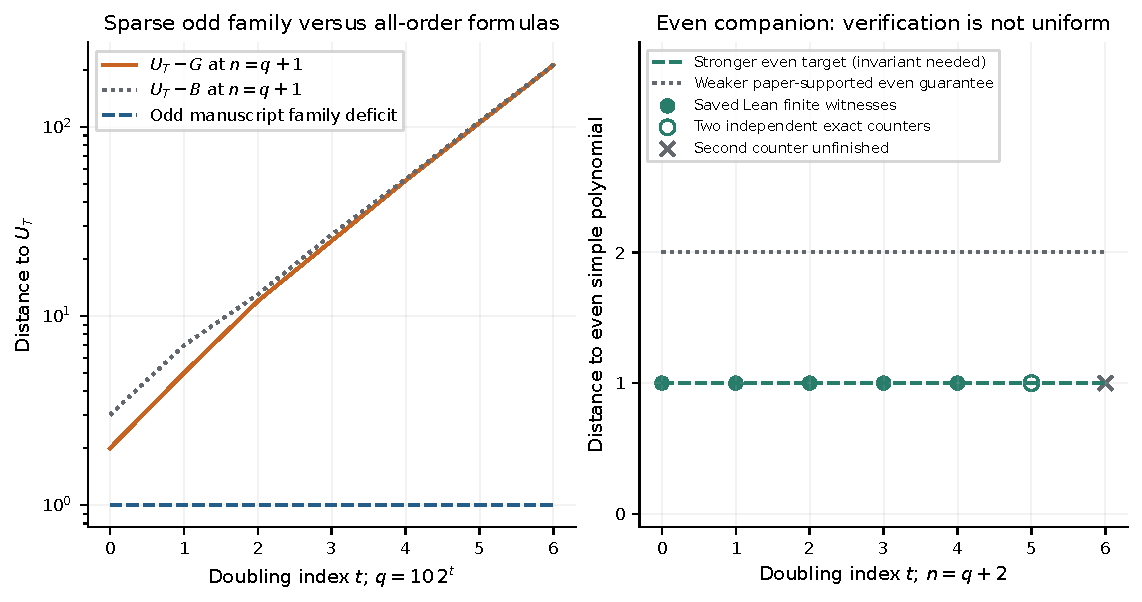
\includegraphics[width=0.88\linewidth]{figures/family-deficits.pdf}
\caption{The original sparse-family deficit plot, retained as a historical
numerical figure. Its arithmetic is unchanged. The family formulas now
have completed Lean existence proofs; any finite-check status encoded
in the original plot describes the September coordinate artifacts. The
new figure below compares the completed envelope.}
\label{fig:family-deficits}
\end{figure}

The independent adjacency and half-plane counters agree on the archived
321-, 322- and 641-line coordinate files, with $34132$, $34292$ and
$136532$ triangles. Their largest rational components have 916, 985 and
1103 decimal digits. The 642-line file passed adjacency and simplicity
checks but its separate direct recount was interrupted. That coordinate
artifact still has partial computational status. In contrast, existence
of some 642-line simple arrangement with at least $136852$ triangles is
now proved by Theorem~\ref{fam:even-conditional}. An existential proof
does not retrospectively certify the exact bytes of a saved coordinate
file.

\subsection{An improved verified bound at every natural order}

Recall the previous retained bound $\Lbound(n)=\max\{G(n),C(n)\}$ in
\eqref{eq:envelope}. Define the sparse family contribution
\begin{equation}
 R(n)=\begin{cases}
 (q_t^2-4)/3,& n=q_t+1,\\
 (q_t^2-4)/3+q_t/2,& n=q_t+2,\\
 0,&\text{otherwise},
 \end{cases}
 \qquad q_t=10\cdot2^t,
 \label{fam:sparse-bound}
\end{equation}
and put
\begin{equation}
 H(n)=\max\{\Lbound(n),R(n)\}.
 \label{fam:new-envelope}
\end{equation}
The two cases have different parity and each determines $t$ uniquely.
The executable Lean definition uses the maximum of the candidates for
$0\le t\le n$, rather than an infinite search.

\begin{theorem}[Total retained and recursive envelope]\label{fam:all-n-envelope}
For every $n\in\N$, $\K(n)\ge H(n)\ge\Lbound(n)$. For every $t\ge5$,
\begin{align}
 H(q_t+1)-\Lbound(q_t+1)&=\floor{q_t/3}-2,\\
 H(q_t+2)-\Lbound(q_t+2)&=q_t/2-\floor{q_t/3}-2,
 \label{fam:exact-gains}
\end{align}
and both differences are positive.
\end{theorem}
\begin{proof}
Each nonzero candidate in \eqref{fam:sparse-bound} has a simple witness
by the preceding two theorems, hence an unrestricted witness. The
finite maximum chooses one such witness or a retained finite/baseline
witness; it is not an addition of incompatible triangle counts. If a
candidate occurs at order $n$, then $t<2^t\le n$, so the executable
finite maximum includes it. This is
\proofref{Kobon/RecursiveEnvelope.lean}{51}{\lean{all_n}}.

Since $q_t^2\equiv1\pmod3$ and $q_t$ is even, substitution in $G$ gives
\[
 T_t-G(q_t+1)=\floor{q_t/3}-2,\qquad
 T_t+q_t/2-G(q_t+2)=q_t/2-\floor{q_t/3}-2.
\]
All saved finite enhancements end at order 195. Thus
$\Lbound(n)=G(n)$ for $n>195$, as proved by
\lean{BBLFamilyBenchmarks.previous_envelope}. For $t\ge5$,
$q_t\ge320$ and both differences are positive. The formal strict-tail
statement is \lean{RecursiveEnvelope.strict_previous_tail}; uniqueness
of the sparse candidate identifies $H$ with that candidate here.
\end{proof}

At 321 and 322 lines the gains over the old verified envelope are
respectively 104 and 52; at 641 and 642 they are 211 and 105. The first
members do not displace stronger retained certificates: $21:133$,
$22:143$, $41:533$ and $42:553$ remain in $H$. All 138 coordinate
identities and their published attribution are retained. This theorem
improves the previous verified repository envelope at infinitely many
orders. It does not prove a numerical record against all published
families, and its off-family values retain the preceding all-order
linear deficit.

\begin{figure}[tb]
\centering
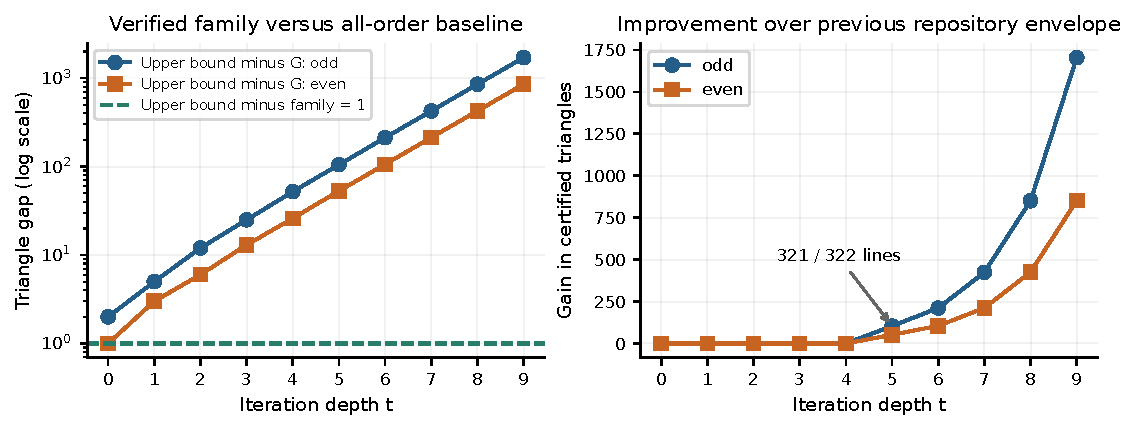
\includegraphics[width=0.95\linewidth]{figures/recursive-envelope.pdf}
\caption{The completed recursive family and the retained all-order bound.
The improvement is over the previous repository envelope; it is not a
numerical-priority comparison against all published constructions. The
upper comparisons refer to simple arrangements. Formula values are
proved in Lean; the plot is newly generated from those formulas.}
\label{fig:recursive-envelope}
\end{figure}

\subsection{Actual one-triangle optimality windows}

The October release also closes the geometric upper-bound bridge for
simple arrangements, as proved in Section~\ref{upper:simple-actual}.
This upgrades a comparison with a polynomial to a statement about the
actual extremal quantity.

\begin{corollary}[Simple optimality windows]\label{fam:optimality-windows}
For $q=10\cdot2^t$ and $t\ge0$, write $A=(q^2-4)/3$. Then
\begin{equation}
 A\le\Ks(q+1)\le A+1,\qquad
 A+q/2\le\Ks(q+2)\le A+q/2+1.
 \label{fam:windows}
\end{equation}
\end{corollary}
\begin{proof}
The lower halves are the constructed witnesses. For every simple
arrangement, the geometric upper results give
$3T\le n(n-2)$ and, for even $n\ge4$, $6T\le n(2n-5)$.
Substitution gives respectively
\[
 \floor{(q+1)(q-1)/3}=A+1,
 \qquad \floor{(q+2)(2q-1)/6}=A+q/2+1.
\]
The exact combined declarations are
\proofref{Kobon/BBLFamilyOptimality.lean}{29}{\lean{odd_window}} and
\proofref{Kobon/BBLFamilyOptimality.lean}{35}{\lean{even_window}}.
\end{proof}

The upper halves use standard logical axioms only; the lower halves
retain their seed's native dependencies. This one-triangle interval
need not be sharp at the smaller orders: the literature settles some
of them more precisely. In particular it is not an upper theorem for
arrangements with multiple concurrence, and it does not close the
unrestricted Kobon problem.

\subsection{Known optimal families and independent reproduction}

The classical dyadic five-line family must be kept separate from the
new compatible eleven-line realization.  A convenient normalized seed
uses intercepts $(-1,-\varepsilon,\varepsilon,1)$ and
\[
 x-v_jy=a_j,\qquad (v_0,v_1,v_2,v_3)=(-15,10,-10,30),
\]
together with $Y_0$.  The complete interval
$0<\varepsilon\leq10^{-5}$ has five certified triangles, all three
distinguished triangles, and two visible pairs.  Its central slopes
are $1/10$ and $-1/10$; the rightmost slope is $1/30$.
The normalization is deliberate: an earlier affine-equivalent numerical
realization had both central slopes negative, which was inadequate as
an unchecked premise for the sign convention in the published iterative
proof.  The corrected whole-parameter seed is verified in
\texttt{TamuraSeed5}.

The known optimal odd family and its simple even companions have
\begin{equation}
 q=4\cdot2^t,\qquad
 \Ks(q+1)\geq\frac{q^2-1}{3},\qquad
 \Ks(q+2)\geq\frac{q^2-1}{3}+\frac q2.
 \label{fam:tamura}
\end{equation}
The current finite certificates include
$5:5$, $6:7$, $9:21$, $10:25$, $17:85$, $18:93$, $33:341$,
$34:357$, $65:1365$, $66:1397$, $129:5461$, and $130:5525$.
These reproduce known numerical consequences of the affine family of
Forge and Ram\'irez Alfons\'in and BBL's odd-to-even discussion
\cite{forge1998,bbl2008}; they are not claimed as newly discovered
bounds.  Theorem~\ref{fam:doubling} as currently formalized does not
cover the small bases $q=4,8,16$, and the unfinished large parametric
33-line draft is not counted as a completed theorem.

Parpalak and Utkin supply a different straight-line family at
$q=18\cdot2^t$~\cite{parpalakutkin2026}.  Its odd count is
\begin{equation}
 \Ks(q+1)\geq\frac{q^2}{3}-1,
 \label{fam:pu}
\end{equation}
including $19:107$ and $37:431$.  The present work independently checked
their compatible 19-line seed on $0<\varepsilon\leq10^{-3}$ with 1632
exact endpoint determinant checks, a rational 107-triangle witness,
and all 17 distinguished triangles.  The interval reproduction is
separate from an end-to-end Lean proof of their infinite construction.
Both the seed and the family retain Parpalak--Utkin attribution.
The earlier BBL statement at $18\cdot2^t+1$ concerned pseudolines;
it cannot be used as a straight-line result without a realization
argument.  Applying Corollary~\ref{ext:odd-full} to the published
straight-line family gives the attributed simple even corollary
\[
 \Ks(q+2)\geq\frac{q^2}{3}+\frac q2-1,
\]
with $20:116$, $38:449$, $74:1763$, and $146:6983$.  Stronger nonsimple
published values at some of these orders concern $\K$, and do not
invalidate this simple-arrangement distinction.

\subsection{The former integration gap and the remaining seed branches}

The verified 21-line base has the true tangent intercepts
\eqref{fam:old-grid} with $q=20$, fixed rational slopes, 132 triangles,
19 distinguished triangles, ten visible pairs, and the required
rightmost-line property for every $0<\varepsilon\le10^{-5}$.
Its finite interval checks use native evaluation; their analytic and
geometric soundness proofs are proved separately.

\begin{figure}[tb]
\centering
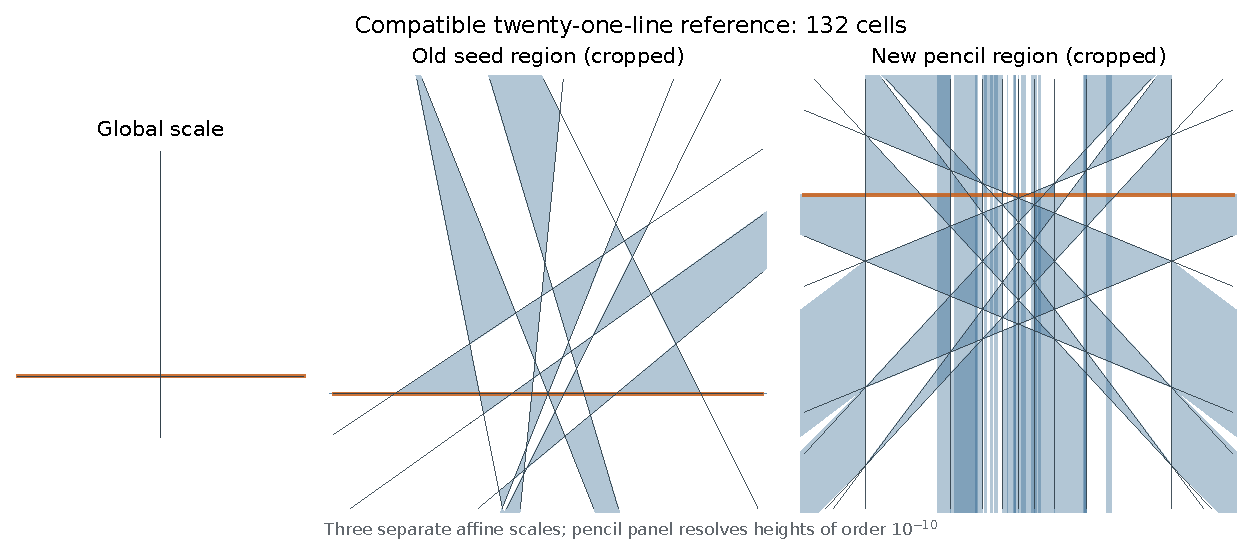
\includegraphics[width=0.88\linewidth]{figures/seed-21.pdf}
\caption{A 21-line hybrid checkpoint with 132 triangles. The global,
core and thin-pencil views illustrate scale separation. The finite
rendering is distinct from the true-tangent-grid parametric theorem in
\lean{BBLSeed21}. The normalized seed now starts the fully verified
recursion; the picture is not used as its proof.}
\label{fig:seed21}
\end{figure}

The September manuscript correctly identified four missing interfaces:
retained geometric data, whole-list transport under the next-grid
permutation, normalization of the 21-line grouped labels, and induction
on a positive parameter interval. All four are now complete. The
central source labels 5 and 6 have apex height $5\varepsilon/2$;
normalization preserves that actual point. The next central triangle
is retained independently of whether it appears in the counted list.
The invariant used in the successful induction is
\begin{equation}
 \exists\eta>0\quad\forall\varepsilon\in(0,\eta)\quad
 \exists\text{ a compatible counted seed at }(q,\varepsilon).
 \label{fam:recursive-quantifier}
\end{equation}
The former target
\begin{equation}
 q_t=20\cdot2^t,\qquad
 \Ks(q_t+1)\ge\frac{q_t^2-4}{3}
 \label{fam:21-target}
\end{equation}
is therefore a theorem, the tail of \eqref{fam:eleven-family}. The
visible-boundary interfaces are also closed by the same release.

This completion does not discharge every possible concrete seed.
For the Forge--Ram\'irez Alfons\'in branch, the active
\lean{BBLForgeConditional} proves the generic formulas
\[
 \Ks(32\cdot2^t+1)\ge\frac{1024\cdot4^t-1}{3},\qquad
 \Ks(32\cdot2^t+2)\ge\frac{1024\cdot4^t-1}{3}+16\cdot2^t
\]
under the explicit premises \texttt{UniformSeed 8 341} and its visible
analogue. The large concrete 33-line uniform base and its dependent
sources remain excluded drafts: the full native check did not finish.
Finite certificates at 33, 34, 65, 66, 129 and 130 remain valid. A
finite base at one parameter is not the uniform base premise above.

\subsection{A uniform 49-line compatibility certificate}
\label{fam:seed49}

The October search found a stronger compatible seed at order 49 using
fixed rational reciprocal slopes of denominator $10^{10}$. Its 48
intercepts are
\[
 -\tan\frac{23\pi}{48},\ldots,-\tan\frac\pi{48},
 -\varepsilon,\varepsilon,
 \tan\frac\pi{48},\ldots,\tan\frac{23\pi}{48}.
\]
Exact rational interval arithmetic verifies, throughout
$0<\varepsilon\le1/100$, a simple arrangement with 767 certified
triangles, all 47 distinguished-line caps and a positive central apex.
The fixed normal $(1,-2)$ has 24 visible pairs, including rightmost
pair $(0,48,49)$; the last slope is $1/3$ and the required boundary
inequalities hold uniformly. These are exact external certificate
claims, not completed finite Lean base theorems.

The analytic part is now inside Lean:
\sourcefile{Kobon/BBLTangent48Bounds.lean}{\lean{BBLTangent48Bounds}}
proves rational enclosures for each of the 23 positive tangent values,
using half-angle and reciprocal identities beginning with
$\tan(\pi/3)=\sqrt3$. The endpoint widths are at most
$5\cdot10^{-36}$. The exported finite predicates were independently
replayed: 1,176 direction checks, 18,424 simplicity checks, 37,583
triangle/support checks and 1,176 visibility/support checks passed.
Two independent exact cell counters also find 767 triangles at the
rational midpoint witness. None of these facts is a substitute for the
unfinished Lean evaluation of the full parametric base.

\begin{figure}[tb]
\centering
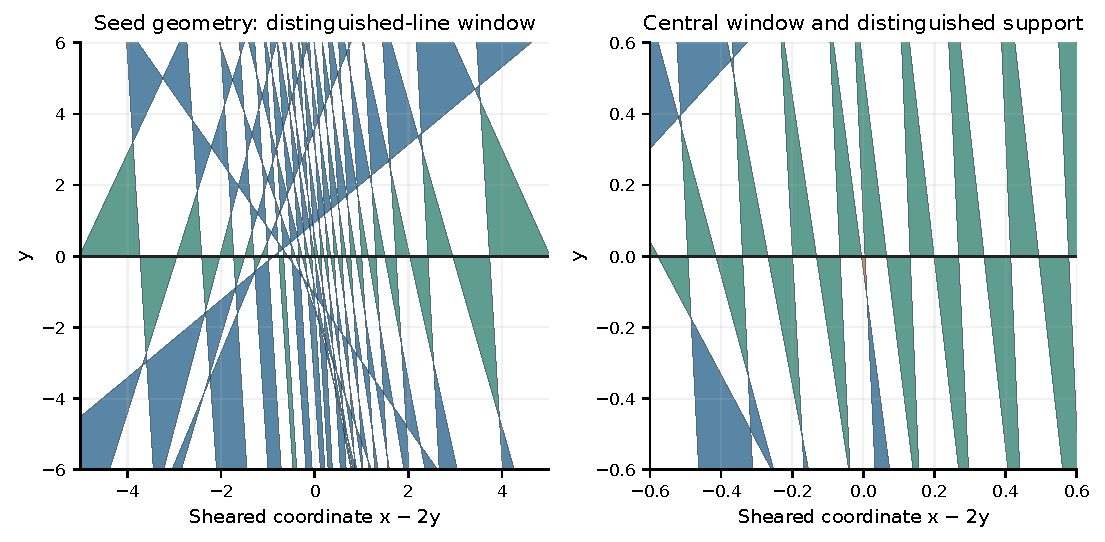
\includegraphics[width=0.98\linewidth]{figures/uniform49.pdf}
\caption{Two clipped windows of the rational midpoint witness for the
uniform 49-line seed, with $\varepsilon=1/200$. The invertible shear
$x'=x-2y$ makes the distinguished structure easier to see. The left
window has $x'\in[-5,5]$, $y\in[-6,6]$; the right has both coordinates
in $[-0.6,0.6]$. Ordinary certified cells are blue, distinguished caps
teal and the central cell orange. Distant cells lie outside these
windows: the panels do not display all 767 triangles. The uniform
certificate is exact external evidence; full Lean seed integration
remains incomplete.}
\label{fig:uniform49}
\end{figure}

If this uniform seed is promoted into the proved recursive interface,
its counts will be
\begin{equation}
 q=48\cdot2^t,\qquad T_{\rm odd}=768\cdot4^t-1,
 \qquad T_{\rm even}=768\cdot4^t+24\cdot2^t-1
 \label{fam:49-conditional}
\end{equation}
at orders $q+1$ and $q+2$. The odd formula is exactly the tail $s=t+3$
of BBL's Theorem~1.3 for $n=6\cdot2^s+1$~\cite{bbl2008}; these are
not new numerical records. The contribution of this branch is an
explicit, well-conditioned uniform compatibility certificate and a
partially completed formal linkage. Five dependent seed/family files
are visibly excluded as unverified drafts. Isolated tangent, graph and
arithmetic proofs do not make the full base proof complete.

Earlier positive-margin fits had moved triangles across infinity.
The successful fit additionally preserves the original affine sign
system. This illustrates why incidence or a projective order type alone
cannot certify the desired affine cell count.

A preceding search for a perfect compatible 21-line seed tested
11,547,910 floating proposals and 3,234 linear-feasibility programs
without improving 132. Those bounded failures were not impossibility
proofs. The exact obstruction in Section~\ref{exp:grid-obstruction}
now proves a much more precise limitation for a prescribed grid and
supplied classification; it still does not exclude other compatible
families or a different geometric construction.
